\chapter{Contributions}

While Julia produces usually faster code than other languages at the same abstraction level for numerical application, the true power of the language is only shown when the programmer writes the code following a couple performance tips listed on the official documentation. One of the most commonly occurring mistake that results suboptimal code is the high number of automatic memory allocations that leads to more frequent calls to garbage collector, and in other words, it wastes resources. Therefore in the following presentation of the programming-related contributions we will highlight the memory-efficiency at the evaluation of the created code base.

\section{FunctionOperators package}

As we have seen so far in the descriptions of the algorithms, operations very often are expressed as a multiplication a matrix-like entity and a vector or matrix. That notation is particularly convenient as it allows using the same set of mathematical tools as we have for matrices, while allows extension of the capabilities of the conventional linear mapping defined as a matrix-vector multiplication. In practice that means that we would like to combine the flexibility of functions with the power of tools designed for matrices, so many times the best option is to define the operation we want to perform as a function, and then wrap this function in an object that acts like a matrix and therefore it is compatible for instance with iterative solvers like the conjugate gradient method. Also it is desirable to add an "backward" operation, also defined by a function, to that wrapper object, that defines what should the solver do when it wants to use the adjoint of the operator.

Being driven by mostly scientists, the Julia community has already developed some packages that helps keeping the code structurally and visually similar to the abstract mathematical notation; nevertheless, none of these were completely satisfying. In particular, there are three relatively popular packages that have such functionality, but all of them some drawbacks:
\begin{itemize}
    \item LinearOperators.jl~\cite{noauthor_juliasmoothoptimizerslinearoperatorsjl_2020} and LinearMaps.jl~\cite{jutho_jutholinearmapsjl_2020} aims to provide almost all features of general matrices, but this design choice restricts the possible inputs to vectors.
    \item AbstractOperators.jl~\cite{noauthor_kul-forbesabstractoperatorsjl_2020} is a fairly new package that overcomes this limitation and provides a relatively large range of features, mostly in the form of predefined operators for the most common operations such as DFT, convolution, finite differences etc. It is also memory effective, preallocating a buffers when two operators are composed (that corresponds to the matrix-matrix multiplication) and it reuses this buffer later avoiding unnecessary memory allocations. Unfortunately, this optimization makes it impossible to accept on GPU arrays that makes unfavorable for large-scale applications.
\end{itemize}

As Julia is designed to be very extendable, it is always a feasible option to develop a new package that fits the specific problem. After reviewing the code of the mentioned packages, we came to the conclusion that the design choices of these packages doen't allow addition of features we desired, without breaking the already existing features, we decided to implement a package that fits better the image CS-MRI reconstruction framework. The developed package is named FunctionOperators.jl and it is already published to the central Julia package repository. Being just after the initial phase, the package supports only the most basic features, but the design of the interface and the efficient implementation lets the user build arbitrarily complex composite operators without having any computation penalty compared to the implementation with pure functions. As of today, the already implemented features if the package are the following:
\begin{itemize}
    \item Construction from a function with one argument that defines "forward" operation. When the constructed FunctionOperator is being multiplied with a vector/matrix of the \textit{proper} size, this function is called on the given vector/matrix. The size of the \textit{proper} input and expected output is a mandatory argument of the constructor of FunctionOperator, and any input with a mismatching size is rejected, and it after the multiplication the size of the output is also checked against the output size specified at construction. E.g., the following code calculates the FFT of x and stores in y:\\
    \lstinline{ Op = FunctionOperator(forw = x -> fft(x))}\\
    \lstinline{ y = Op * x}
    \item Construction from two functions both accepting one argument. These functions define the "forward" and the "backward" operations. In contrast to the "forward" function, the "backward" function is called when adjoint of the FunctionOperator is requested. E.g., the following calculates the inverse FFT of x and stores in y:\\
    \lstinline{Op = FunctionOperator(forw = x -> fft(x), backw = x -> ifft(x))}\\
    \lstinline{y = Op' * x}
    \item These "forward" and "backward" functions also can accept two arguments. In that case, the second argument is the input of the operation, and the functions are expected to store the result of the operation in the first argument. This feature is advantageous if one wants to optimize the number of memory allocations. E.g., the following multiplies x elementwise with two and stores the result in y without allocating an intermediate array.\\
    \lstinline{Op = FunctionOperator(forw = (b,x) -> b .= x .* 2)}||
    \lstinline{mul!(y, Op, x)} 
    \item Composition of FunctionOperators by multiplication (that means composition of the "forward" functions), addition and substraction (these adds/substracts the output of the operations). E.g. considering the following the last line evaluates to true:\\
    \lstinline{Op1 = FunctionOperator(forw = x -> fft(x))}\\
    \lstinline{Op2 = FunctionOperator(forw = (b,x) -> b .= x .* 2)}\\
    \lstinline{Op1 * Op2 * x == fft(x .* 2)}
    \item Composition of FunctionOperators with UniformScaling object from LinearAlgebra standard library. This UniformScaling operator corresponds to the identity matrix. E.g. we can define the MR acquisition operator $\mathcal{A}$ as a FunctionOperator, and then we can define the CG operator in algorithm~\ref{alg:al-cg} as $\mathcal{A}' * \mathcal{A} + \delta_1 I$ (it is not the abstract mathematical notation, but a valid Julia expression because Julia also accepts Unicode characters in the identifiers!) and then we can pass it to a a solver (IterativeSolver.jl has, for example, CG solver that uses duck-typing, so it requires only that the multiplication must be implemented on the object passed as argument).
    \item Adjoint of composit FunctionOperators: If the FunctionOperator is a composition of other FunctionOperators, then the adjoint is defined as the composition of adjoints of the member FunctionOperators, in the reverse order. E.g., let us recall the decomposition of the acquisition operator $\mathcal{A} = \Omega \mathcal{FC}$. Now look on it on the other way around: we have $\Omega, \mathcal{F}$ and $\mathcal{C}$ already created as FunctionOperators, and we create the acquisition operator as the composition of them: $\mathcal{A} = \Omega * \mathcal{F * C}$. Then $\mathbf{A}' * x$ would do the same as $\mathcal{C' * F'} * \Omega' * x$.
\end{itemize}

Under the hood, the most important property of the package that it uses the least amount of memory possible by deferring the allocation of buffers as much as possible and also by maintaining a smart global pool that stores the already allocated buffers. These buffers are only needed to store intermediate results, and therefore they are safe to reuse in different FunctionOperators provided that they are on the same thread. But the user don't need to worry about that criterion since this case is handled automatically, making FunctionOperators a thread-safe package (assuming that the user builds the operators from thread-safe "forward" and "backward" functions). This memory effective implementation makes FunctionOperators a truly unique as other packages are all more or less suboptimal in this sense.

As an extra (yet experimental) feature, FunctionOperators package provides a macro that automatically optimizes loops by cutting down the number unnecessary memory allocations. To achieve this the macro uses the advanced code generation features that produces code before the compilation of the program, but after the parser has built the abstract syntax tree and deduced the type of variables; therefore, heavy optimizations can be performed behind the scenes using macros and generated functions. %Fig.~\ref{} shows three versions of the same code fragment: one is a readable version that resembles the mathematical formulation, the other is a memory-wise optimal, but much less readable code, and the third one show the usage of the macro that reduces the amount of allocated memory by $~70\%$.

Following the guidelines of the Julia community for package development, the code is thoroughly tested using unit tests, and has a clean documentation that contains a notebook with an example for almost all features. The coverage of unit tests are measured by \url{codecov.io}, and it reported that the $94\%$ of the code is covered. This report, however, underestimates the coverage as it fails to detect the covered lines in case of tests checking the functions that prints to console. The code of the package is uploaded to \url{https://github.com/hakkelt/FunctionOperators.jl}, and the documentation is available at \url{https://hakkelt.github.io/FunctionOperators.jl/latest/}.

\section{Implementation of Sparse+Low Rank algorithms}

After the careful examination of both the publication and the reference Matlab implementation, we created an efficient Julia version for each of these algorithms. As the implementation was done at the same time as the FunctionOperators was developed, it was a natural choice to benchmark the newly developed package against the other similar packages on these algorithms. The contribution of this part of the project is two-fold: First, it extends the currently small code base of MRI-related algorithms in Julia, helping the fast growing group of scientists choosing to prototype their research algorithms in Julia. Second, it might also help those who needs guidance in picking the right package, especially because currently no other comparison is available to see the difference between LinearMaps.jl and AbstractOperators.jl.

The result of the benchmarking is available in table~\ref{tab:lin_fessler} and the Jupyter notebooks holding both the benchmarking code, the documentation, and the results are available at \url{https://github.com/hakkelt/reproduce-l-s-dynamic-mri-julia}
In comparison to the Matlab implementation, the results are somewhat mixed since Julia outperformed Matlab in case of the improved AL scheme (the speedup here was ~2x) and in case of proximal methods for the non-Cartesian dataset (with 2-3.5x speedup). On the other hand, Matlab produced faster code for the other cases. This results underlines the fact that merely switching the language to Julia not necessarily results in increased speed automatically. A possible explanation is that we missed some hidden optimization tricks deeply buried in the Matlab code (which was well optimized indeed, and very hard to read---it required a fair amount of time from us to understand how is it connected to the theory described in the paper). Another possible factor is that Matlab uses some proprietary C and fortran libraries that have slightly better performance compared to the open source options bundled with Julia by default.

Furthermore, the comparison of different Julia implementations revealed that the three package have very similar running time (that matches our expectations as these packages are meant to be "invisible" in performance benchmarks being only wrappers around some functions), but they rahter differ in the memory allocated, LinearMaps.jl having the largest memory demand (as it was expected from the implementation that allocates and releases buffers in each iteration again and again in our case), and FunctionOperators being better than AbstractOperators by a small margin. We also tested the automatic optimization macro mentioned above, and the benchmarks showed that it reached almost optimal memory usage, reducing the size of net allocations by $~70\%$ on average, compared to the $~80\%$ reduction achieved by the tedious process of manual optimization.

\begin{table}
\footnotesize
\begin{tabular}{|p{0.1\linewidth}|p{0.18\linewidth}p{0.18\linewidth}p{0.18\linewidth}p{0.18\linewidth}|}
\hline
algorithm \textbackslash data set & PINCAT & Multicoil cardiac cine MRI & Multicoil cardiac perfusion MRI & Multicoil abdominal dce MRI \\ \hline
\multicolumn{1}{|c|}{} & \multicolumn{4}{c|}{Matlab} \\
AL-CG & 16.8 s & 49.0 s & 19.9 s & - \\
AL-2 & 17.8 s & 55.3 s & 27.5 s & - \\
ISTA & 1.7 s & 5.5 s & 2.3 s & 141.8 s \\
FISTA & 2.4 s & 7.6 s & 3.1 s & 256.7 s \\
POGM & 1.8 s & 5.8 s & 2.3 s & 140.0 s \\ \hline
\multicolumn{1}{|c|}{} & \multicolumn{4}{c|}{LinearMaps} \\
AL-CG & 28.4 s, 11.26 GiB & 80.8 s, 31.08 GiB & 33.8 s, 12.95 GiB & - \\
AL-2 & 9.8 s, 6.22 GiB & 28.4 s, 17.56 GiB & 11.0 s, 7.32 GiB & - \\
ISTA & 6.0 s, 627.71 MiB & 19.6 s, 1.36 GiB & 6.8 s, 582.06 MiB & 72.7 s, 2.18 GiB \\
FISTA & 6.2 s, 627.71 MiB & 16.5 s, 1.36 GiB & 6.8 s, 582.06 MiB & 73.2 s, 2.18 GiB \\
POGM & 6.3 s, 677.71 MiB & 16.8 s, 1.45 GiB & 6.8 s, 622.06 MiB & 72.6 s, 2.42 GiB \\ \hline
\multicolumn{1}{|c|}{} & \multicolumn{4}{c|}{AbstractOperators} \\
AL-CG & 28.7 s, 678.06 MiB & 76.1 s, 1.45 GiB & 32.1 s, 622.41 MiB & - \\
AL-2 & 9.0 s, 1.14 GiB & 23.3 s, 2.93 GiB & 10.2 s, 1.22 GiB & - \\
ISTA & 6.4 s, 627.68 MiB & 16.4 s, 1.36 GiB & 7.3 s, 582.03 MiB & 72.8 s, 2.18 GiB \\
FISTA & 6.5 s, 627.68 MiB & 16.3 s, 1.36 GiB & 7.3 s, 582.03 MiB & 72.0 s, 2.18 GiB \\
POGM & 6.6 s, 677.68 MiB & 16.5 s, 1.45 GiB & 7.0 s, 622.03 MiB & 73.9 s, 2.42 GiB \\ \hline
\multicolumn{1}{|c|}{} & \multicolumn{4}{c|}{FunctionOperators naive} \\
AL-CG & 30.6 s, 2.90 GiB & 79.4 s, 6.14 GiB & 33.3 s, 2.43 GiB & - \\
AL-2 & 11.6 s, 12.20 GiB & 32.0 s, 33.17 GiB & 13.1 s, 13.82 GiB & - \\
ISTA & 6.8 s, 3.40 GiB & 18.1 s, 8.67 GiB & 7.6 s, 3.62 GiB & 72.7 s, 6.71 GiB \\
FISTA & 6.9 s, 3.40 GiB & 17.6 s, 8.67 GiB & 7.5 s, 3.62 GiB & 74.9 s, 6.71 GiB \\
POGM & 6.9 s, 3.45 GiB & 17.8 s, 8.77 GiB & 7.5 s, 3.65 GiB & 73.741 s, 6.96 GiB \\ \hline
\multicolumn{1}{|c|}{} & \multicolumn{4}{c|}{functionOperators optimized} \\
AL-CG & 27.0 s, 640.69 MiB & 76.2 s, 1.38 GiB & 33.0 s, 592.54 MiB & - \\
AL-2 & 8.6 s, 1.04 GiB & 22.7 s, 2.65 GiB & 10.0 s, 1.11 GiB & - \\
ISTA & 6.1 s, 627.79 MiB & 16.6 s, 1.36 GiB & 7.6 s, 582.14 MiB & 75.1 s, 2.18 GiB \\
FISTA & 6.1 s, 627.79 MiB & 16.5 s, 1.36 GiB & 7.9 s, 582.14 MiB & 73.8 s, 2.18 GiB \\
POGM & 6.3 s, 677.79 MiB & 16.747 s, 1.45 GiB & 7.079 s, 622.14 MiB & 73.6 s, 2.42 GiB \\ \hline
\multicolumn{1}{|c|}{} & \multicolumn{4}{c|}{FunctionOperators pretty} \\
AL-CG & 28.0 s, 741.02 MiB & 75.1 s, 1.57 GiB & 30.7 s, 662.87 MiB & - \\
AL-2 & 8.4 s, 1.26 GiB & 21.8 s, 3.26 GiB & 9.3 s, 1.36 GiB & - \\
ISTA & 6.3 s, 1.05 GiB & 16.4 s, 2.49 GiB & 6.9 s, 1.04 GiB & 73.5 s, 3.03 GiB \\
FISTA & 6.3 s, 1.05 GiB & 16.3 s, 2.49 GiB & 6.9 s, 1.04 GiB & 72.2 s, 3.03 GiB \\
POGM & 6.4 s, 1.10 GiB & 16.5 s, 2.58 GiB & 6.9 s, 1.08 GiB & 74.5 s, 3.28 GiB \\ \hline
\end{tabular}
\caption{Benchmarking on different datasets performing reconstruction via proximity and augmented Lagrangian methods descirbed in~\cite{lin_efficient_2019}. "FunctionOperators naive" is an implementation with minimal manual optimizations, "FunctionOperators optimized" is a manually optimized version, and ""FunctionOperators pretty" is exactly same as the "naive" version except that our automatic automatic optimizer macro is called on the code.}
\label{tab:lin_fessler}
\end{table}

\section{Implementation of Multiscale Decomposition}

The implementation of multiscale low rank algorithm described in~\cite{ong_extreme_2020}, posed multiple challenges. First, the algorithm was written in a framework, also developed by the author, called SigPy~\cite{noauthor_sigpy_nodate}. Practically that meant that we needed to re-implement a fairly large part of that library in Julia. While it would have been possible to directly call the methods from this framework, these blocking would make the paralellization of the Julia code practically impossible. The other largest challenge was that the author used a special version of the non-uniform FFT (NFFT), also from his package, and therefore we also needed to re-implement this non-trivial method as well because it was not compatible with the Julia implementation of NFFT. However, this difficulty later turned out to be beneficial, as we realized a performance problem in the author's code, and correcting it in our implementation doubled its speed. But first let us discuss shortly the NFFT algorithm.

\subsection{NFFT}
As the name suggests, non-uniform FFTs are the non-Cartesian variant of the FFT, and therefore they are very useful in MRI reconstruction with real-life data. Also, similarly to the FFT which is the fast version of DFT, non-uniform FFT is also derived from non-uniform DFT. There are many possibilities how to calculate them efficiently, but the most widely used variant is proposed by Fessler~\cite{fessler_nonuniform_2003}. This variant maps the off-grid coordinates determined by the non-Cartesion trajectory to the closest grid point and to its neighbor pixels, using a kernel (most commonly the Kaiser-Bessel function) to weight this projection. Then, it applies the ordinary FFT to the grid filled with values by the mapping. Finally, it utilizes some technique, known as apodization in the photography, that corrects the artifacts introduced by the undersampling and the mapping to the grid. The large popularity of this approach is that there are many highly optimized FFT solutions, and therefore the speed of NFFT only depend on the effective mapping (the time complexity of apodization is negligible compared to the mapping).

In our implementation we used the FFTW library to compute the FFT, which is currently the fastest open source solution (and some even claim that it outperform the commercial ones). This library supports also multithreading that help us also speeding up the code. When we compared our implementation to the implementation in SigPy, we considered three multithreading settings: a fully singly threaded, a partially single threaded (the Julia code is single threaded, and the multithreading in FFTW is allowed), and a fully multithreaded. Concerning the size of the problem: We tested the implementation for three sizes, a small sized random image ($64\times64$) and relative few sampling points ($1024$), a "medium sized" where the image were relatively large with size of $128\times128\times128$, but the number of sampling point were still low compared to the size of the image ($16k$ sampling points), and the "large" problem where the image size is reduced to keep the problem feasible, but the number of sampling points were large. In case of the "medium" and "large" data, a batch dimension of size $12$ is also provided that means that no Fourier transformation is done along that direction, but the same operation takes place on each slice defined by this direction.

The numerical results, then showed us that the best multithreading setting is depends on the problem, as we expected. Moreover, the multithreading in FFTW brings larger benefits when the size of input image is large (in these cases the FFT is the dominant step in the NFFT), while enabling the Julia multithreading (these threads then distributes the sampling between each other) has a large positive impact when the number of sampling points are sufficently large (let's say over $1M$ points). In the MRI cases, the latter is not an infrequent situation. For a better insights to the results, we refer the reader to fig.~\ref{fig:nfft_small}-\ref{fig:nfft_large}. In these figures we show two different versions of the Julia implementation: one contains the initialization steps, the other not. While the former is good enough when we want to evaluate the NFFT only once, the latter is good when we perform the same operation multiple times; e.g., in a loop. In these cases, one might want to avoid repeated allocations in the initialization part, and therefore our implementation makes it possible to create a \textit{plan} and then apply this plan to the data avoiding the repeated initialization.

%\subsection{Optimization possibilities}
%\begin{enumerate}
%    \item Batch-processing: compute NUFFT of all channels at once
%    \item Parallelization:
%    \begin{enumerate}
%        \item NUFFT
%        \item Algorithm
%    \end{enumerate}
%    \item GPU-specific optimizations:
%    \begin{enumerate}
%        \item Blocking operator might cause CPU bottleneck
%    \end{enumerate}
%\end{enumerate}

%\subsection{Parallelization Solution}
%Details how I made the code run parallel

\begin{figure}[htbp]
    \centering
    \begin{minipage}{0.48\linewidth}
        \centering
        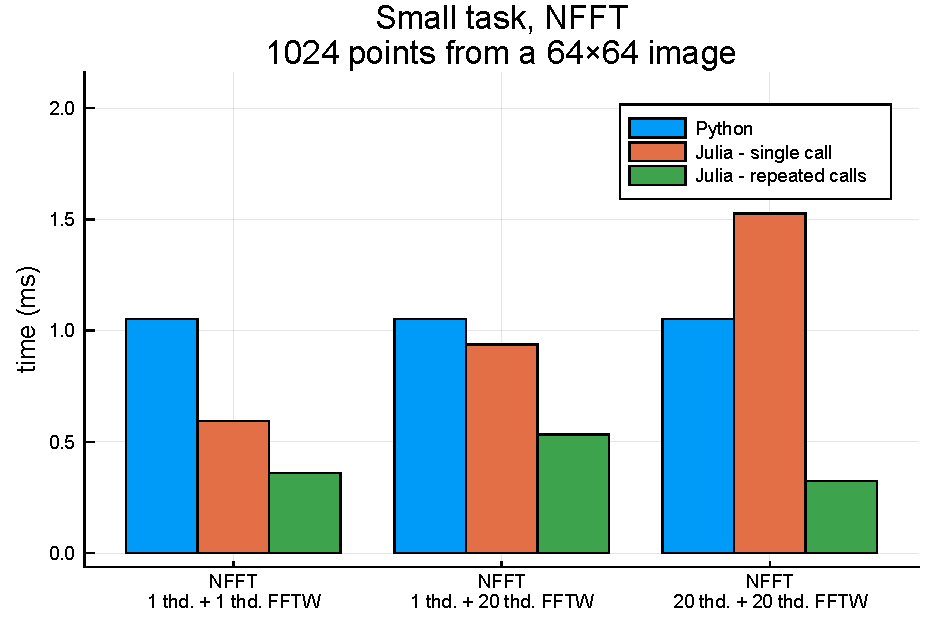
\includegraphics[width=\linewidth]{images/nfft_small_forw.pdf}
        \label{fig:nfft_small_forw}
    \end{minipage}
    \begin{minipage}{0.48\linewidth}
        \centering
        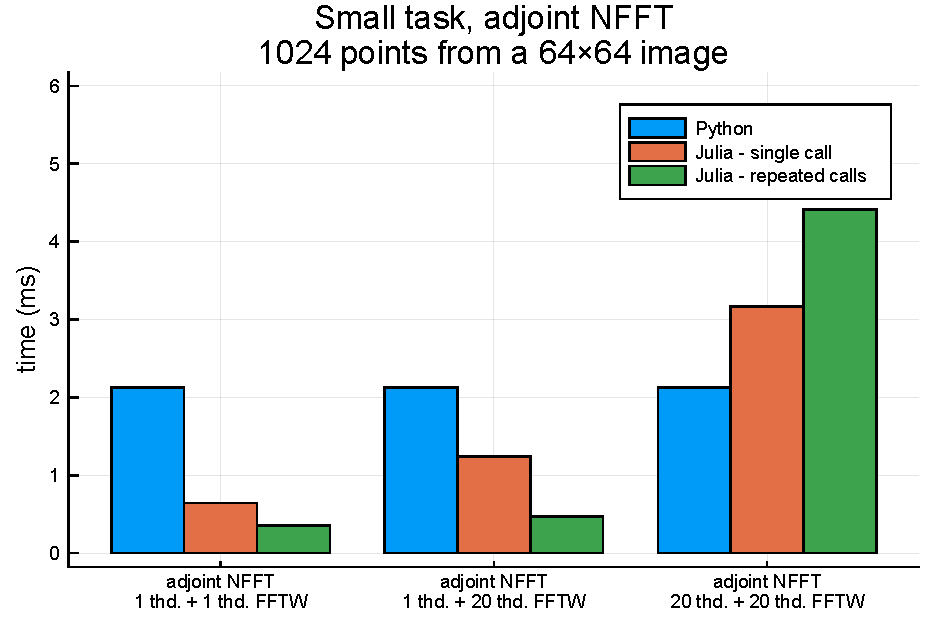
\includegraphics[width=\linewidth]{images/nfft_small_backw.pdf}
        \label{fig:nfft_small_backw}
    \end{minipage}
    \caption{\textbf{Comparison of running time} between the Python implementation in SigPy package (blue), and the Julia implementations (orange: initialization and computation), green: computation only) at different threading settings \textbf{in the case of a small problem} (small input image with relatively few sampling points). \textbf{For small images, single threaded Julia version is the fastest.} (Note that the Python implementation does not implement multithreading, and hence the height of the three blue bar is the same.)}
    \label{fig:nfft_small}
\end{figure}

\begin{figure}[htbp]
    \centering
    \begin{minipage}{0.48\linewidth}
        \centering
        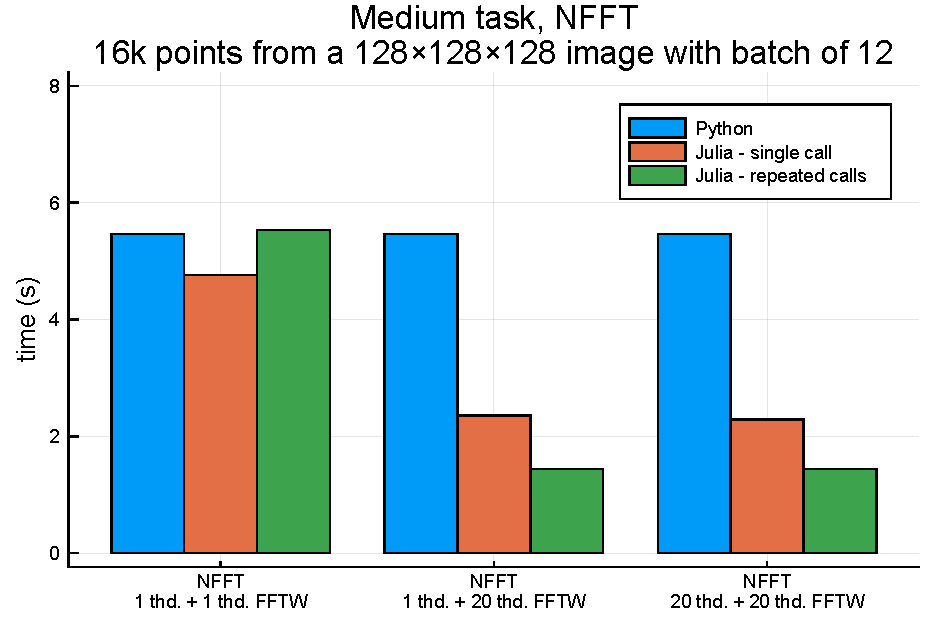
\includegraphics[width=\linewidth]{images/nfft_medium_forw.pdf}
    \end{minipage}
    \begin{minipage}{0.48\linewidth}
        \centering
        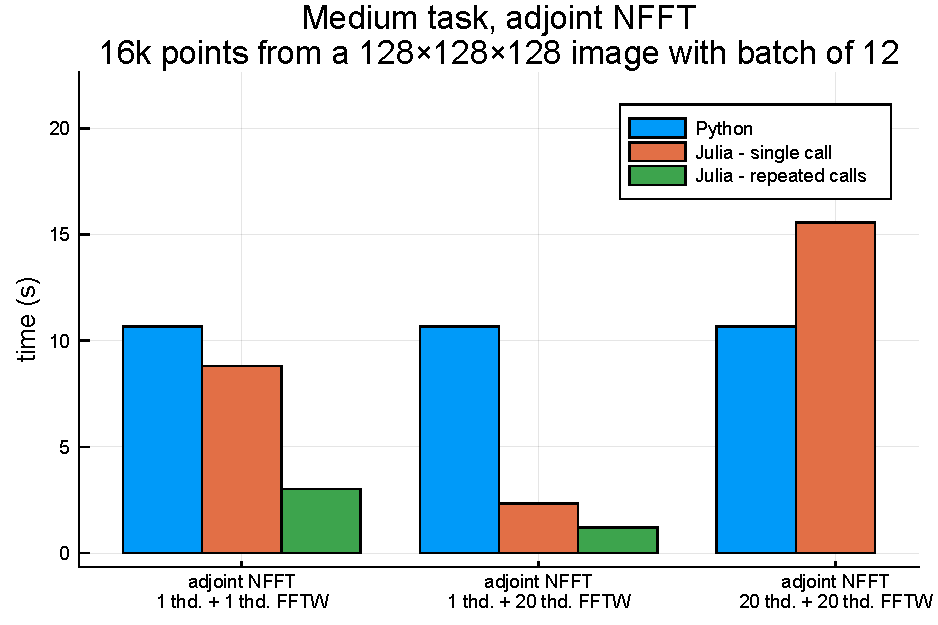
\includegraphics[width=\linewidth]{images/nfft_medium_backw.pdf}
    \end{minipage}
    \caption{\textbf{Comparison of running time}  in the medium sized setting: Single threaded Julia + multithreaded FFTW yielded the best performance.}
    \label{fig:nfft_medium}
\end{figure}

\begin{figure}[htbp]
    \centering
    \begin{minipage}{0.48\linewidth}
        \centering
        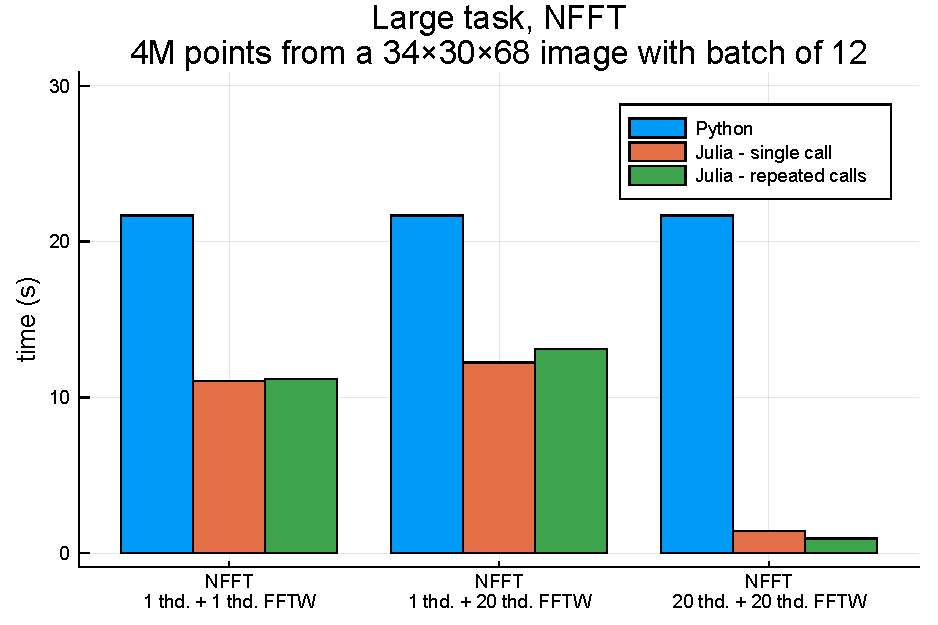
\includegraphics[width=\linewidth]{images/nfft_large_forw.pdf}
    \end{minipage}
    \begin{minipage}{0.48\linewidth}
        \centering
        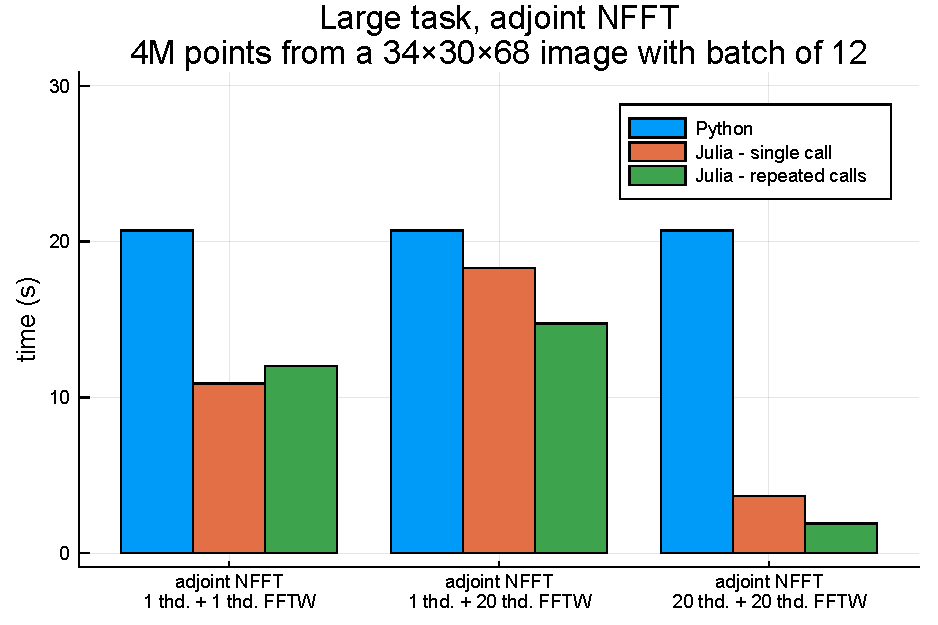
\includegraphics[width=\linewidth]{images/nfft_large_backw.pdf}
    \end{minipage}
    \caption{\textbf{Comparison of running time} in case of large number of sampling points: Multithreaded Julia code + multithreaded FFTW were the fastest.}
    \label{fig:nfft_large}
\end{figure}

\subsection{MSLR Algorithm}

After finishing the re-implementation of the necessary parts of SigPy in Julia, our attention is turned towards the implementation of the algorithm itelf that was not a challenge any more as almost all important operators and functions are defined in SigPy. Being aware of the speedup in case of the re-implementation of the NFFT, we expected similar acceleration. Yet, the result were even better as we predicted. As we already mentioned, the Python implementation did not exploit the potentials in the batch processing in NFFT. Specifically, it is much faster to pass the image the NFFT specifying along which dimension we want to perform the NFFT, than iterating over th batch dimension (= the dimension along which we \textit{do not} want to perform the NFFT) and calling the NFFT on each slice. 

Fig.~\ref{fig:gridding_recon_speed} demonstrates the effect: Here the measured algorithm technically consists only of a loop that iterates over the batch dimension corresponding to the coils sensitivities, and calls NFFT on each. On the other hand, the Julia version passes the entire arraw to NFFT. The result is drastic, $5.5\times$ speedup, even in the fully single threaded case. But when we anable the full multithreading, algorithm appeared to outperform even the Python's GPU version.

Fig.~\ref{fig:MSLR_recon_speed} does not show so much improvement, but still many-fold speedup is experienced, with the fully multithreaded almost reaching the Pyhton's GPU version.

These results suggest that re-implementing the Python'GPU code in Julia would enjoy, maybe not that much, but significant acceleration. For more information concerning the implementational details, we refer the reader to the GitHub repository of the project: \url{https://github.com/hakkelt/extreme_mri_julia}

\begin{figure}
    \centering
    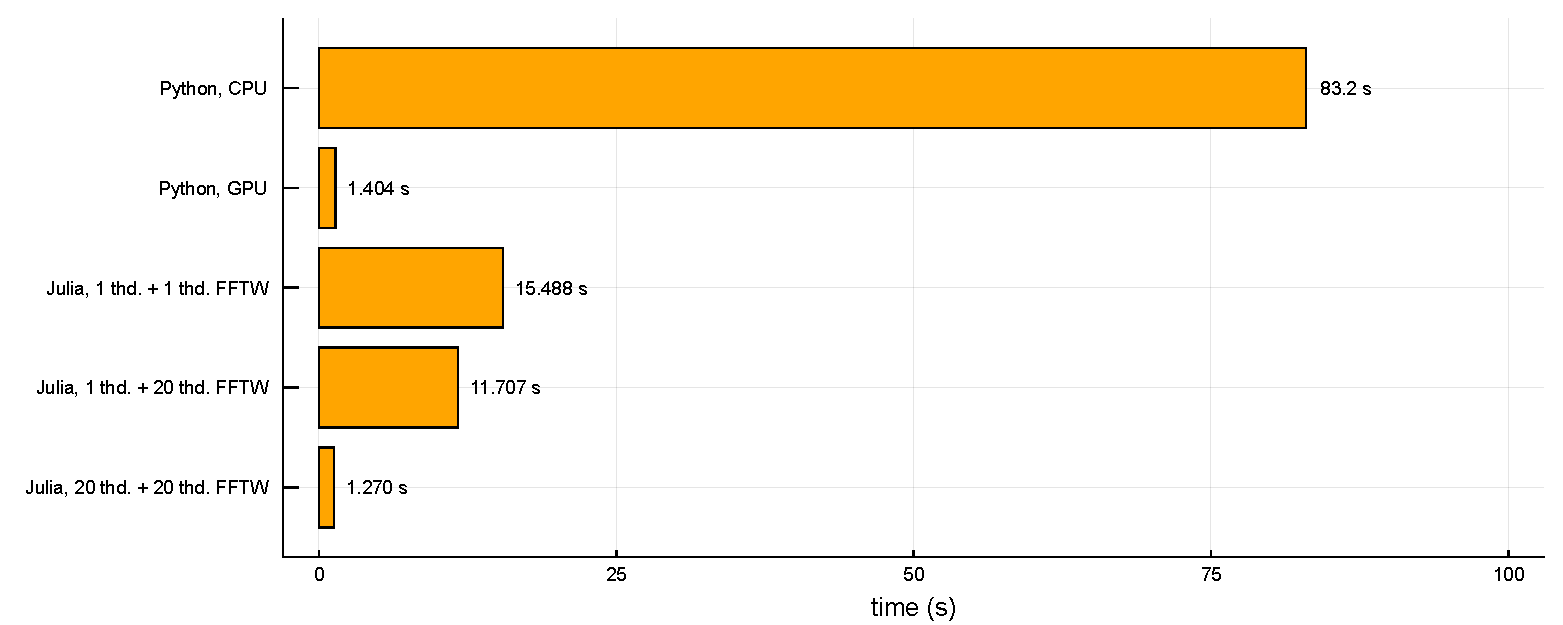
\includegraphics[width=\linewidth]{images/gridding_recon_speed.pdf}
    \caption{Comparison of speed different implementations for the gridding reconstruction problem (i.e. a large scale adjoint NFFT with batch dimensions).}
    \label{fig:gridding_recon_speed}
\end{figure}

\begin{figure}
    \centering
    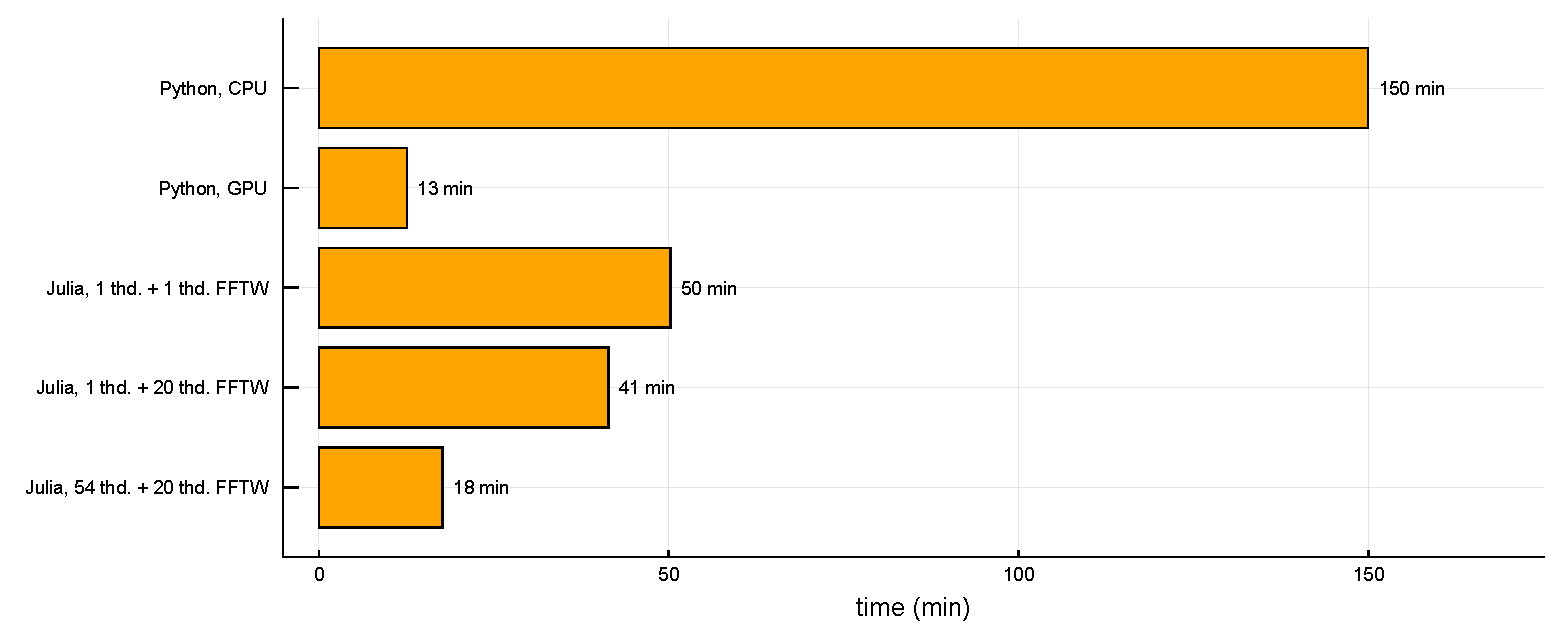
\includegraphics[width=\linewidth]{images/MSLR_recon_speed.pdf}
    \caption{Comparison of speed for different implementation of the MSLR algorithm. Note that the heavily multithreaded Julia implementation was almost as fast as the Python GPU implementation. Also even the fully single threaded Julia implementation was more than three times faster than the Python CPU implementation.}
    \label{fig:MSLR_recon_speed}
\end{figure}

%\begin{figure}
 %   \centering
%    \caption{asdf}
 %   \label{fig:3D_recon}
%\end{figure}

\section{HM-IRLS Implementation}

While the plan at the beginning of the project was to apply the new HM-IRLS method to the $L+S$ problem, the robust version of this algorithm is still not published at the time of the writing, unfortunately. Therefore we were limited make experiments with the low-rank-only variant of the algorithm. To make the comparison to the other method somewhat balanced, we used the simulated dataset from~\cite{wissmann_mrxcat_2014}, and we modified it to produce multiple slightly different datasets, and made experiments on how the parameters of these dataset-variant effects the recovery process. That way we could look at the effect of noise, undersampling ratio, and sparseness. By undersampling, of course, we mean here the undersampling \textit{of the Fourier domain}.

The modification process consisted of a singular value hard thresholding that selected the $r$ largest singular values, and discarded all other. As a result, the thresholding produced an image with the desired rank $r$. Next, we subtracted this low-rank approximation from the original image, and we added back the residual after hard thresholding to the low-rank image. The resulted image served then as "ground truth" image, which we undersampled, and added some noise to the undersampled data. The process in a more exact form:
\[\mathbf{L} = SVHT_r(\mathbf{X})\]
and
\[\mathbf{X}_{gt} = \mathbf{L} + HT_s(\mathbf{X} - \mathbf{L}),\]
where $SVHT_r$ is the singular value hard thresholding,
and $HT_s$ is the hard thresholding that discard all, but the $s$ largest values in a matrix. The last step of the construction of the modified setting was the undersampling where we were in full control of the number of sampled point from the Fourier domain.

In the testing stage, we examined how much can the different algorithms reconstruct the "ground truth" from the undersampled, noisy measurement. Our experiments showed that the HM-IRLS algorithm performed extremely well in the noiseless case and when $s = 0$, that is, the ground truth image was only the low rank component. The results also confirms the claims that POGM converges the fast, FISTA and the improved AL being the second fastest, but finally all of the algorithms designed to minimize the $L+S$ cost converged to the same minimizer after a long time. The MSLR algorithm, however, reached a much worse local minimizer than the other algorithms. Even though it might be surprising at first, the difference in the reach optimizer is fairly reasonable as HM-IRLS solved the low-rank minimization directly, the ones with the $L+S$ cost solved a relaxed problem that minimized nuclear norm instead of the rank, and, finally, the MSLR even relaxed the the nuclear norm even further by the Burer-Monteiro factorization to reduce the memory requirement of the algorithm (therefore it is slightly unfair comparison to others which care less about memory consumption). Moreover, we checked the behavior of the rank during the iterations, and we noted that the while the HM-IRLS algorithm decreased the rank gradually, the soft-thresholding-based algorithms reached the target rank very soon, but the overall cost function stopped also at a ligher level. The AL method with CG steps were the only expection, most probably because of the alternating steps working "against" each other. Fig.~\ref{fig:ideal} shows a setting plot were all algorithms successfully converged.

Unfortunately, even relatively low level of noise or small amount of sparsity can make the HM-IRLS fail to converge. Fig.~\ref{fig:orig} displays such a case, that actually corresponds the setting used in the $L+S$ paper we discussed deeper. In that setting, not only HM-IRLS, but also the MSLR algorithm diverges at all $\alpha$ step sizes. This can certainly avoided by adjusting the parameters of the algorithm. After running many measurements we concluded that SNR under approximately 100 dB makes the HM-IRLS fail to converge for most settings (see fig.~\ref{fig:noise_tolerance}. On the other hand, the reconstruction power of HM-IRLS appeared to be much stronger than the others minimizing the nuclear-norm, as it is depicted on fig.~\ref{fig:reconstruction_power}.

It important to note that the results here are promising, but definitely not decisive, as using HM-IRLS in this form in $L+S$ setting is technically modelling error, and also as we tested only on one dataset. One could rather see the efforts presented here as a proof-of-concept that motivates further investigation.

For more information on the implementation details, see \url{https://github.com/hakkelt/IRLS-for-CS-MRI}.

%\subsection{Description of Algorithm}
%\subsection{Implementation Details}

\begin{figure}
    \centering
    \begin{minipage}{0.48\linewidth}
        \centering
        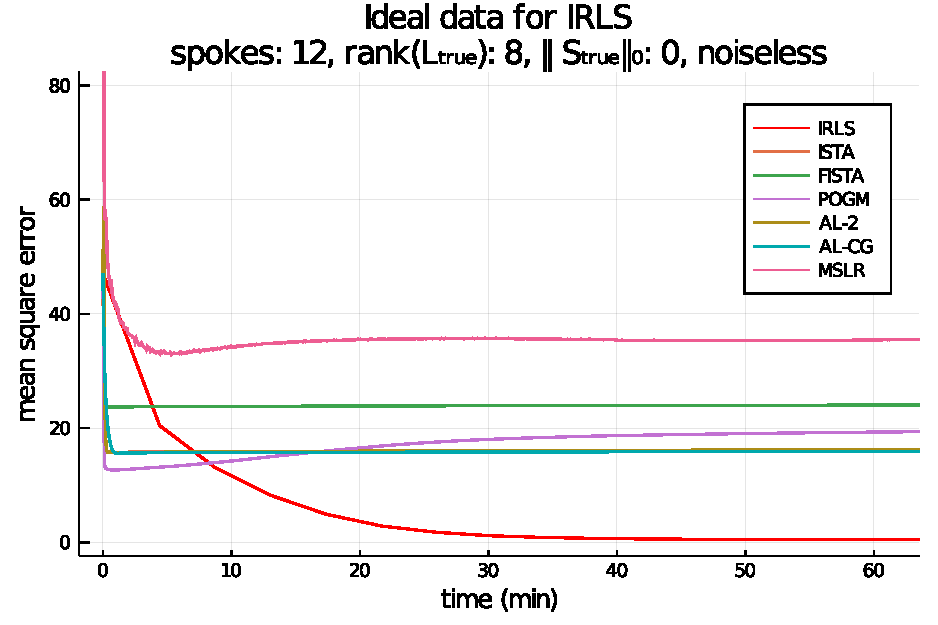
\includegraphics[width=\linewidth]{images/ideal_MSE.pdf}
    \end{minipage}
    \begin{minipage}{0.48\linewidth}
        \centering
        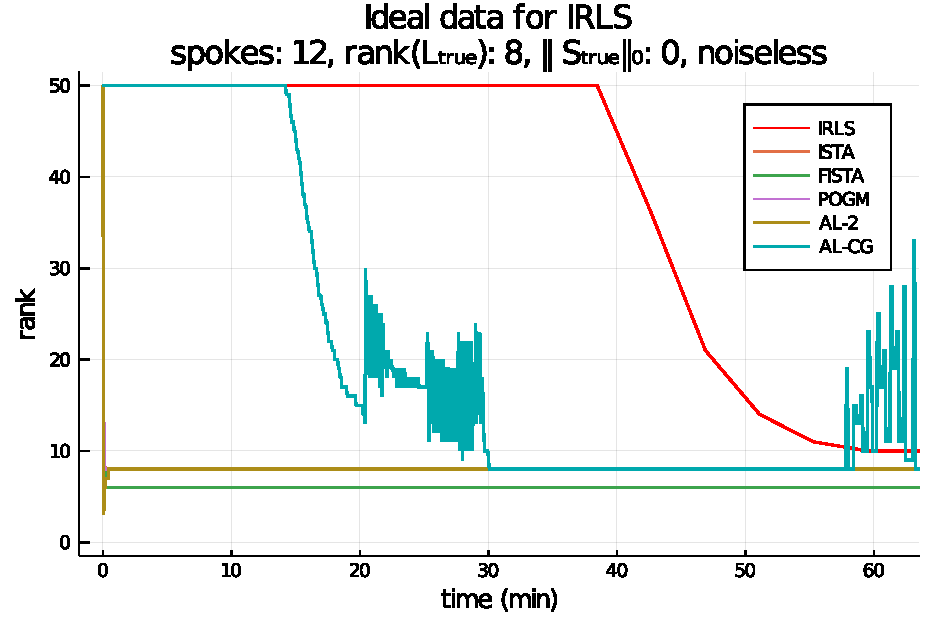
\includegraphics[width=\linewidth]{images/ideal_rank.pdf}
    \end{minipage}
    \caption{\textbf{Ideal case: low-rank only and noiseless} All algorithms converges and HM-IRLS gives the best, almost perfect result. Even tough HM-IRLS seems to be the slowest, in the mathematical sense, it is the fastest. Here on the image the red line shows the result of 30 iterations, while the others perform multiple thousands of iterations. On the right image, showing the rank over the iterations, one can not that HM-IRLS is more careful with decreasing the rank thank other methods, and the decrease is also more smott.}
    \label{fig:ideal}
\end{figure}

\begin{figure}
    \centering
    \begin{minipage}[t]{0.48\linewidth}
        \centering
        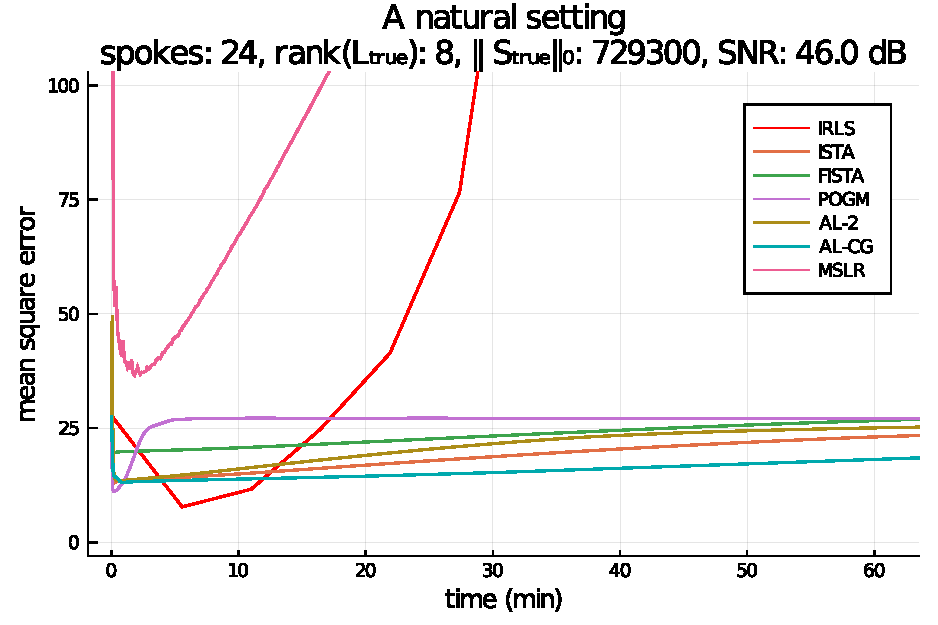
\includegraphics[width=\linewidth]{images/orig_MSE.pdf}
    \end{minipage}
    \begin{minipage}[t]{0.48\linewidth}
        \centering
        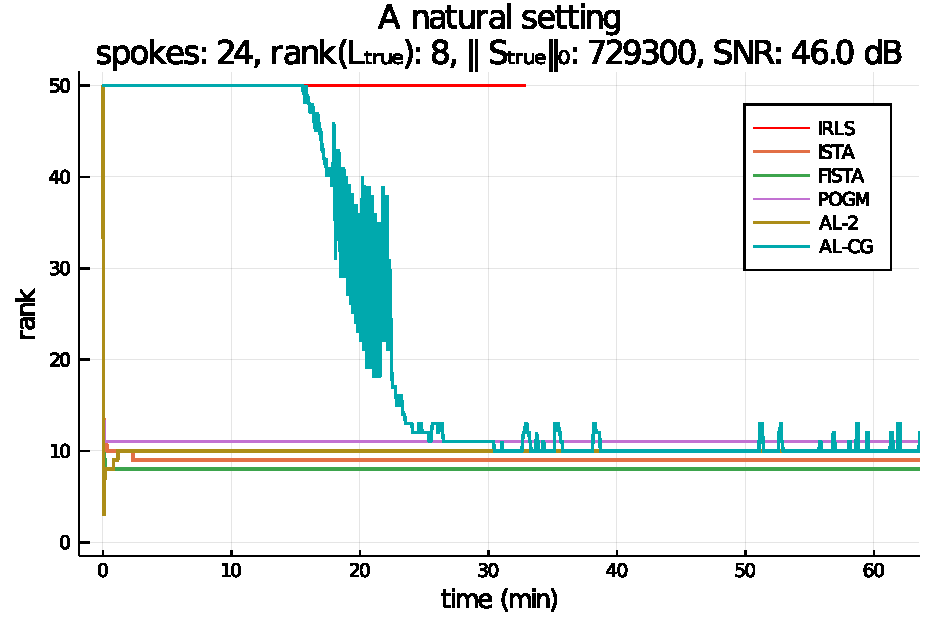
\includegraphics[width=\linewidth]{images/orig_rank.pdf}
    \end{minipage}
    \caption{{Setting that mimics the real-life settings.} HM-IRLS diverges as MSLR also do.}
    \label{fig:orig}
\end{figure}

\begin{figure}
    \centering
    \begin{minipage}[t]{0.48\linewidth}
        \centering
        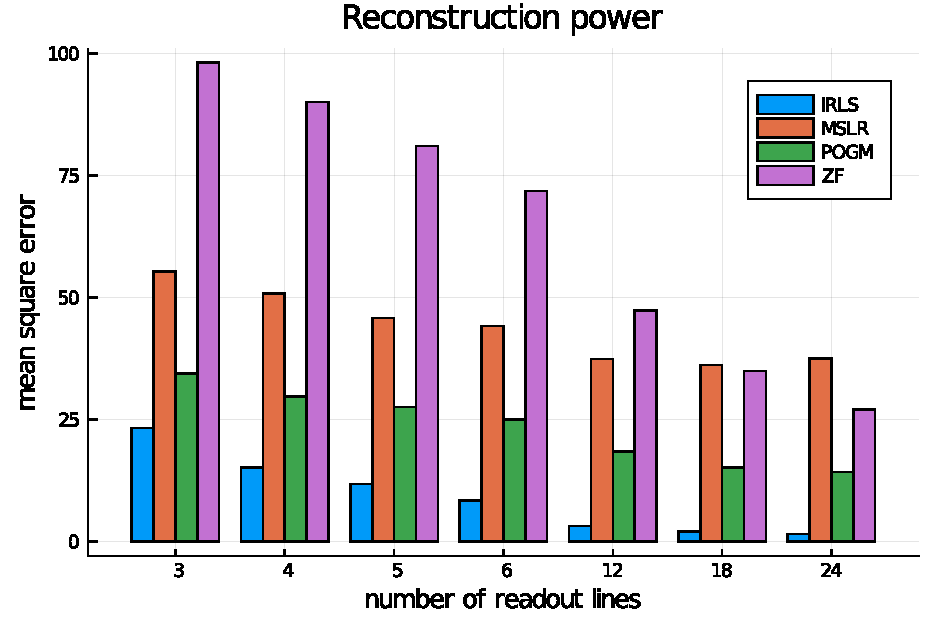
\includegraphics[width=\linewidth]{images/reconstruction_power.pdf}
        \caption{\textbf{Reconstruction power.} The number of measurements (number of "spokes" in the radian sampling trajectory) is increasing resulting more measurement data.HM-IRLS have much better reconstruction in all cases. ZF refers to the naive \textit{zero-filling} method, where the missing values are substituted with zeros.}
        \label{fig:reconstruction_power}
    \end{minipage}
    \begin{minipage}[t]{0.48\linewidth}
        \centering
        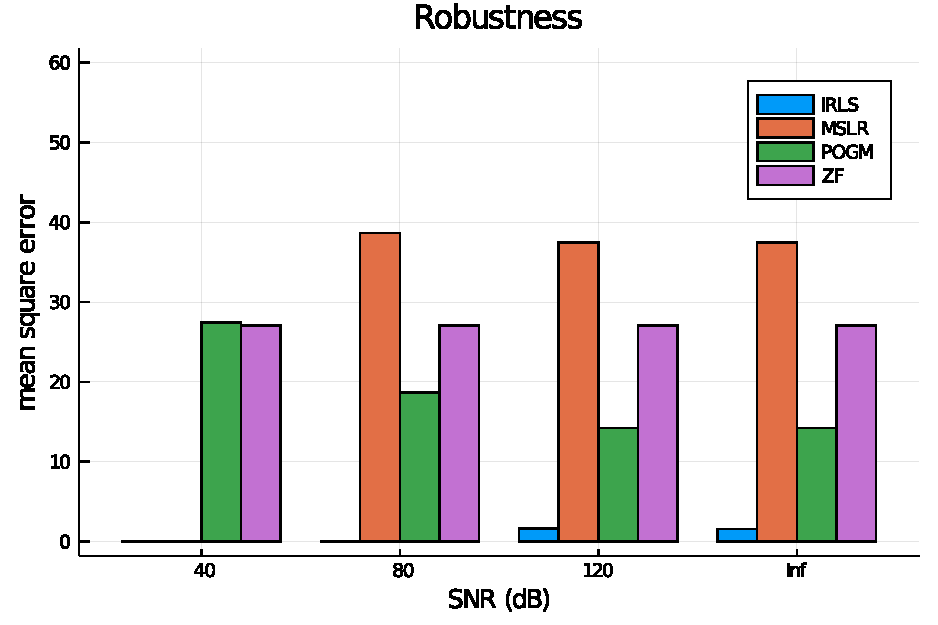
\includegraphics[width=\linewidth]{images/noise_tolerance.pdf}
        \caption{\textbf{Noise tolerance of algorithms.} When the noies is very low, the HM-IRLS gives almost perfect result, but higher noise level quickly degrades the performance. ZF refers to the naive \textit{zero-filling} method when missing values are substituted with ones.}
        \label{fig:noise_tolerance}
    \end{minipage}
\end{figure}

\iffalse
\begin{figure}
    \centering
    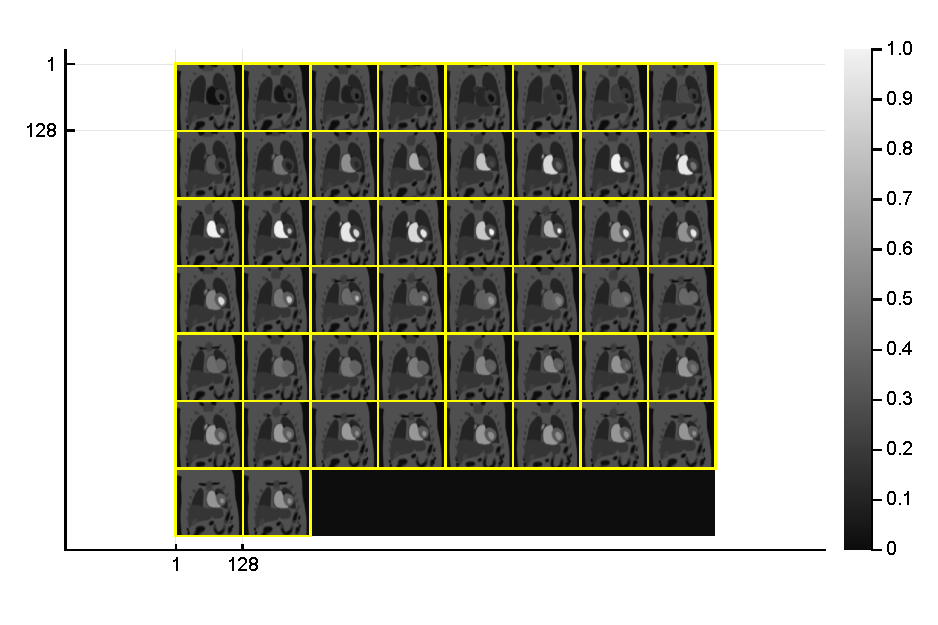
\includegraphics[width=0.46\linewidth]{images/PINCAT_all.pdf}
    \caption{Caption}
    \label{fig:PINCAT_all}
\end{figure}

\begin{figure}
    \centering
    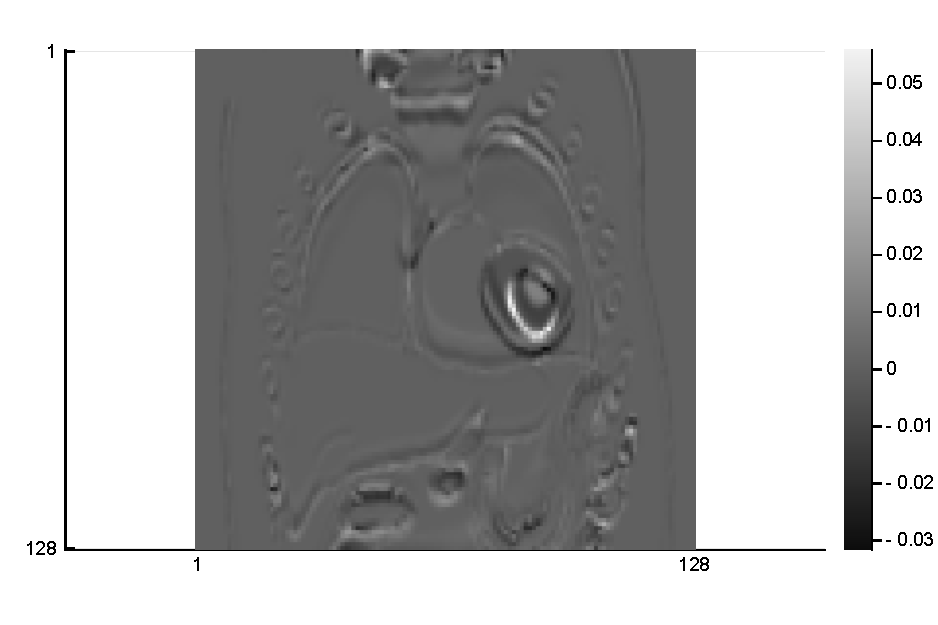
\includegraphics[width=0.46\linewidth]{images/PINCAT_diff_t20.pdf}
    \caption{Caption}
    \label{fig:PINCAT_diff_t20}
\end{figure}

\begin{figure}
    \centering
    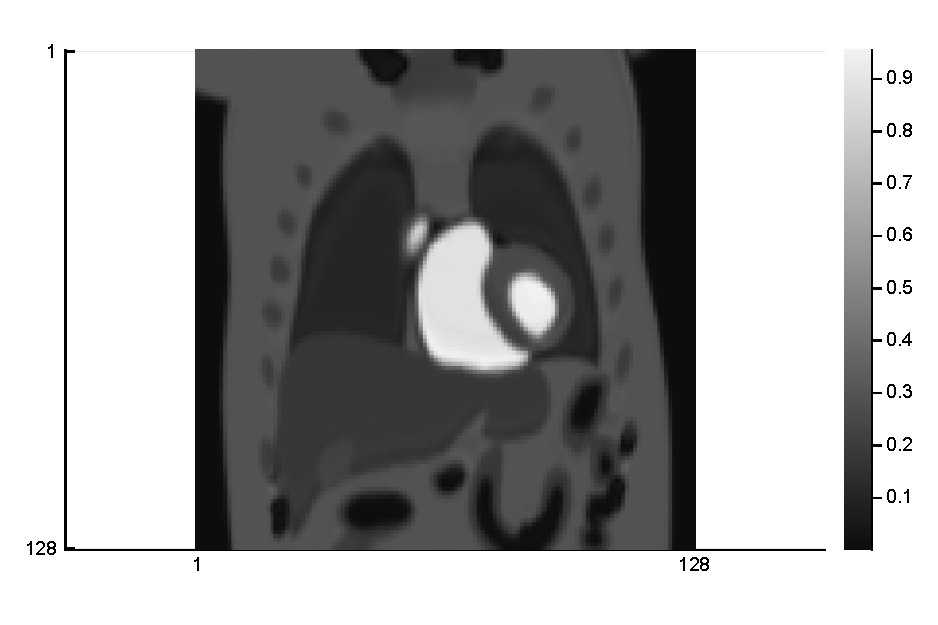
\includegraphics[width=0.46\linewidth]{images/PINCAT_IRLS_recon.pdf}
    \caption{Caption}
    \label{fig:PINCAT_IRLS_recon}
\end{figure}

\begin{figure}
    \centering
    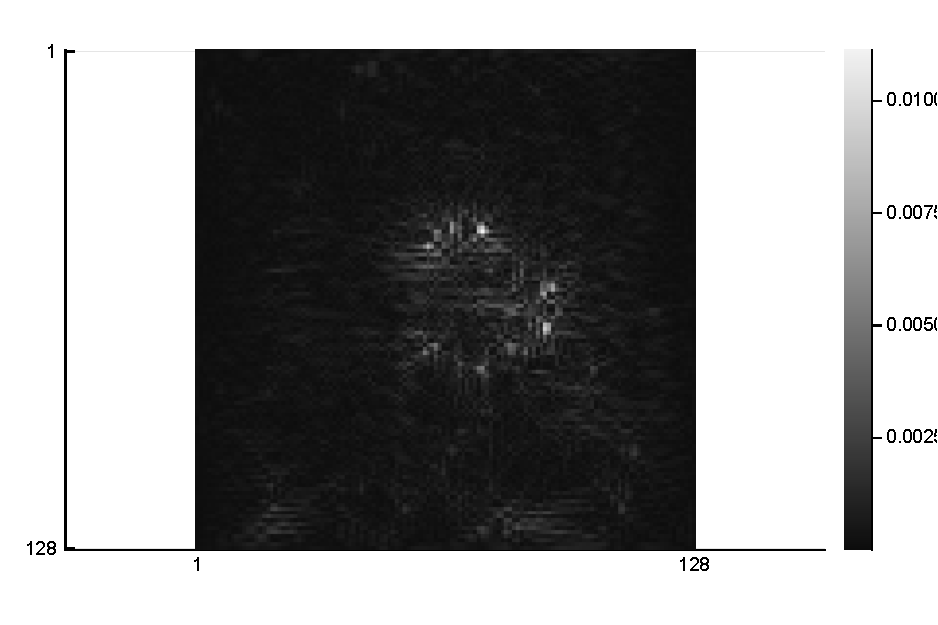
\includegraphics[width=0.46\linewidth]{images/PINCAT_IRLS_recon_error.pdf}
    \caption{Caption}
    \label{fig:PINCAT_IRLS_recon_error}
\end{figure}

\begin{figure}
    \centering
    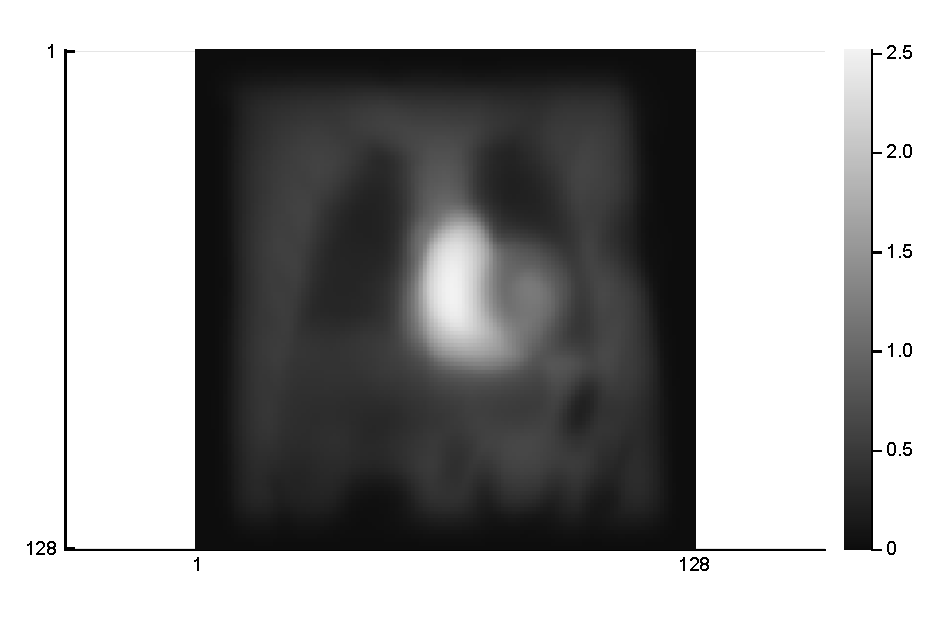
\includegraphics[width=0.46\linewidth]{images/PINCAT_MSLR_recon.pdf}
    \caption{Caption}
    \label{fig:PINCAT_MSLR_recon}
\end{figure}

\begin{figure}
    \centering
    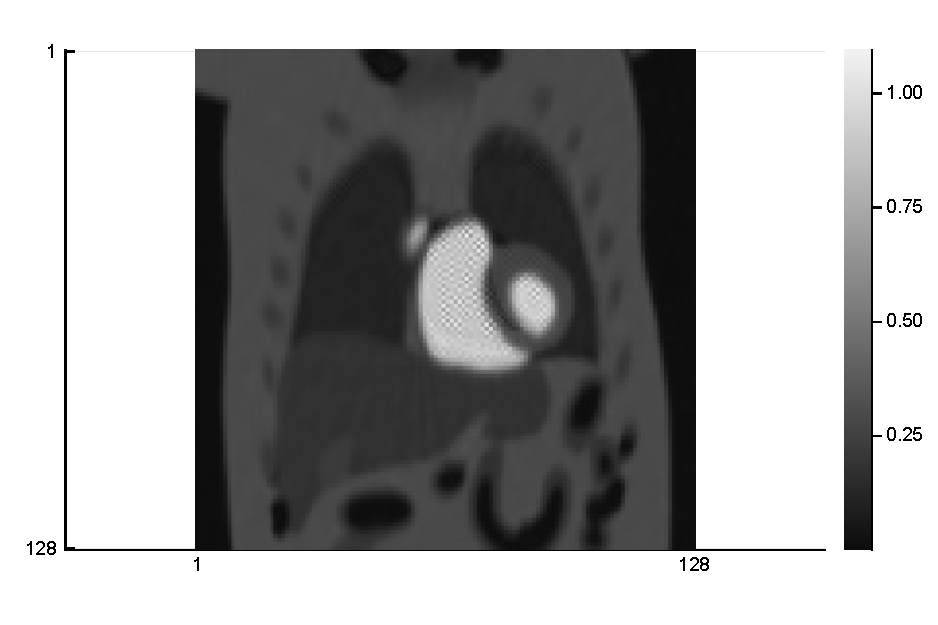
\includegraphics[width=0.46\linewidth]{images/PINCAT_POGM_recon.pdf}
    \caption{Caption}
    \label{fig:PINCAT_POGM_recon}
\end{figure}
\fi

\clearpage % You need \clearpage at the end of every chapter to force images included in this chapter to be rendered in somewhere else
